\section{Resultados}
\label{sec:resultados}

\subsection{Soporte}
\label{sec:res-soporte}

\begin{table*}[tb]
\centering
\caption{\textbf{Hay variación de la corona dentro de celda en los tres tipos de material, y todos los productos con
300 rollos o más tienen soporte para la asociación.} Celdas: producto $\times$ dimensión $\times$ mes. DE corona:
desviación estándar de la corona relativa dentro de celda, en puntos porcentuales del espesor, ponderada por rollos
(celdas con dos o más rollos). Prod.\ $\geq$300: productos con al menos 300 rollos.}
\label{tab:soporte}
\footnotesize
\begin{tabular}{lrrrrrrrr}
\toprule
Tipo & Rollos & Progr. & Prod. & Prod. $\geq$300 & Celdas & \% en celdas $\geq$5 & DE corona (pp) & \% preset 0 \\
\midrule
CALIENTE & 16,456 & 746 & 152 & 12 & 2,070 & 84.6 & 0.69 & 11.6 \\
DECAPADO & 27,177 & 754 & 234 & 23 & 4,457 & 79.6 & 0.53 & 11.1 \\
FRIO & 639 & 121 & 31 & 0 & 136 & 77.2 & 0.38 & 0.0 \\
Total & 44,272 & 831 & 331 & 35 & 6,137 & 83.2 & 0.60 & 11.1 \\
\bottomrule
\end{tabular}

\end{table*}

La Tabla~\ref{tab:soporte} resume el diagnóstico de soporte, hecho antes de cualquier estimación. Los
\NProdGrandes{} productos con al menos 300 rollos reúnen el \PctRollosProdGrandes\,\% de la población y todos tienen
variación de corona dentro de celda; los \NSinSoporte{} productos sin esa variación suman solo \NSinSoporteRollos{}
rollos y salen de la asociación. La corona relativa varía \SDCoronaDentro{}~pp (una desviación estándar) dentro de su
celda, y \PctPresetCero\,\% de los rollos tiene un preset de cero. El análisis de la asociación usa
\NAsocRollos{} rollos en \NAsocCeldas{} celdas con al menos dos rollos y \NAsocProgramas{} programas.

\subsection{De dónde viene la corrección de bending}
\label{sec:res-descomp}

\begin{figure*}[tb]
\centering
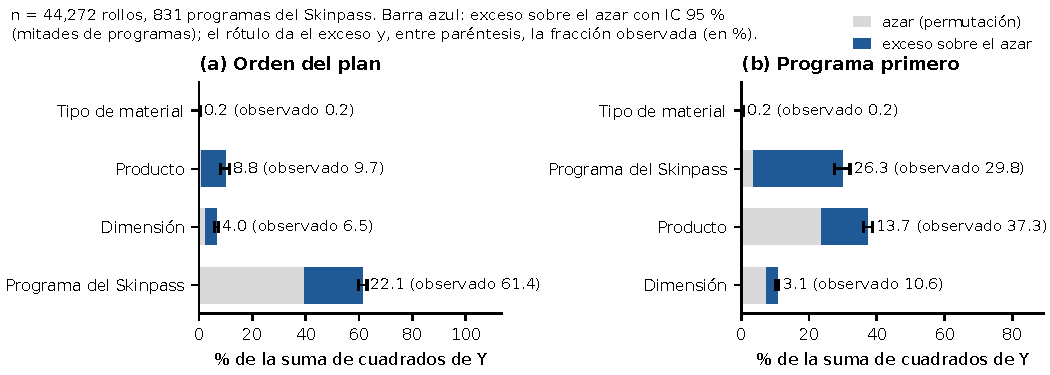
\includegraphics[width=\textwidth]{figuras/fig_r1_descomposicion.pdf}
\caption{\textbf{La corrección de bending varía más entre programas del Skinpass que entre productos, en cualquier
orden de la descomposición.} Pregunta que responde: ¿qué parte de las diferencias de $\Y$ entre rollos se explica por
el tipo de material, el producto, la dimensión y el programa, más allá de lo que daría el azar? Cada barra es la
fracción de la suma de cuadrados de $\Y$ que explica un nivel (ec.~\ref{eq:descomp}); la parte gris es la que el mismo
nivel obtendría con etiquetas permutadas, así que solo cuenta el tramo azul. (a) Orden del plan. (b) Programa antes que
producto.}
\label{fig:descomp}
\end{figure*}

La corrección de bending tiene mediana de \YMediana~kN (percentiles 5 y 95: \YPcinco{} y \YPnoventaycinco~kN): en la
mayoría de los rollos el bending real queda por debajo del preset de la receta. La Fig.~\ref{fig:descomp}
reparte su variación. En el orden del plan, el programa del Skinpass explica \ObsPrograma\,\% de la suma de cuadrados,
pero el azar ya explicaría \NulaPrograma\,\% por el tamaño pequeño de sus grupos dentro de cada producto y dimensión:
su exceso sobre el azar es de \ExcesoPrograma~puntos (IC~95\,\% \ExcesoProgramaIC). El producto aporta
\ExcesoProducto~puntos \ExcesoProductoIC, la dimensión \ExcesoDimension{} \ExcesoDimensionIC{} y el tipo de material
\ExcesoTipo. Producto y dimensión juntos suman \ExcesoProdDim~puntos, menos que el programa solo. Con el programa antes
que el producto (Fig.~\ref{fig:descomp}b), el programa aporta \ExcesoAltPrograma~puntos y el producto \ExcesoAltProducto:
el orden cambia las cifras, pero no cuál pesa más.

\subsection{Corona del MC4 y corrección de bending}
\label{sec:res-corona}

\begin{figure*}[tb]
\centering
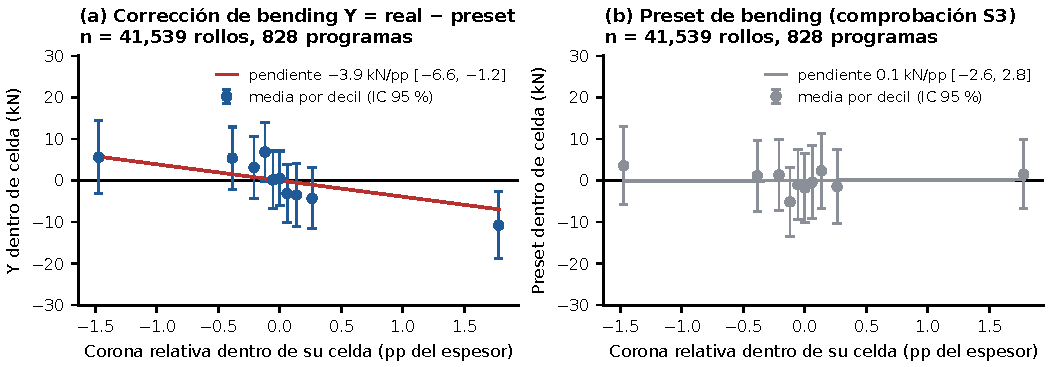
\includegraphics[width=\textwidth]{figuras/fig_r2_corona.pdf}
\caption{\textbf{Más corona relativa de salida del MC4 se asocia con una corrección de bending más negativa, con una
magnitud pequeña; el preset no responde a la corona.} Pregunta que responde: dentro de un mismo producto, dimensión y
mes, ¿los rollos que salen del MC4 con más corona reciben una corrección distinta? Ambos ejes están centrados en la
celda del rollo. Cada punto es la media de un decil de corona, con su IC~95\,\% agrupado por programa; la recta es la
pendiente de la ec.~\ref{eq:fe}. (a) Corrección $\Y$. (b) Preset, como comprobación de que la receta no reacciona a la
corona del rollo.}
\label{fig:corona}
\end{figure*}

Dentro de celda, cada punto porcentual adicional de corona relativa se asocia con una corrección de bending
\PendCorona~kN más negativa (IC~95\,\% \PendCoronaIC; $t=\PendCoronaT$ con errores agrupados por programa), es decir,
\PendCoronaSD~kN por una desviación estándar de corona dentro de celda \PendCoronaSDIC. La corona explica
\RParcialCorona\,\% de la varianza de $\Y$ que queda dentro de celda ($R^2$ parcial). La curva por deciles
(Fig.~\ref{fig:corona}a) es aproximadamente lineal, sin un umbral, y las diferencias entre deciles son de pocos kN.
La desviación de la temperatura de enrollado no se asocia con $\Y$ (\PendTemp~kN por °C, \PendTempIC). El preset no
responde a la corona del rollo (\PendPreset~kN por punto, \PendPresetIC; Fig.~\ref{fig:corona}b).

Con la misma especificación, el bending real se mueve igual que la corrección (\SecBendReal~kN por punto), lo que
descarta que la asociación dependa de las unidades del preset. Los indicadores secundarios no se mueven con la corona:
por cada punto porcentual, el porcentaje de rollos con defecto de inspector cambia \SecDefInsp~puntos porcentuales,
el de rollos retenidos \SecRetenido{} y la elongación lograda \SecElong~puntos de elongación.

\subsection{Heterogeneidad entre productos}
\label{sec:res-het}

\begin{figure}[t]
\centering
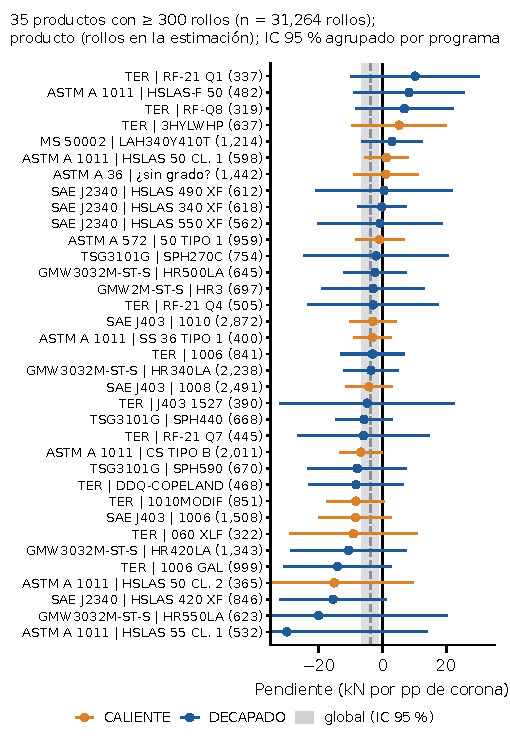
\includegraphics[width=\columnwidth]{figuras/fig_r3_productos.pdf}
\caption{\textbf{Ningún producto muestra una pendiente corona~$\rightarrow$~$\Y$ distinta de cero después de controlar
la tasa de descubrimientos falsos.} Pregunta que responde: ¿la asociación es igual en todos los productos? Cada
renglón es un producto con al menos 300 rollos (entre paréntesis, rollos en la estimación), con su pendiente e
IC~95\,\% agrupado por programa. Están todos, no solo los extremos; la franja gris es la estimación global.}
\label{fig:productos}
\end{figure}

La Fig.~\ref{fig:productos} muestra la pendiente en cada uno de los \NProdHet{} productos con al menos 300 rollos
(\NProdHetRollos{} rollos). \NProdNeg{} de las \NProdHet{} pendientes son negativas, como la global; van de
\PendProdMin{} a \PendProdMax~kN por punto, con intervalos anchos. Solo \NProdICexcluyeCero{} intervalo excluye el cero
y, al controlar la tasa de descubrimientos falsos al 5\,\%, \NProdBH{} productos se distinguen de cero.

\subsection{Validación y sensibilidad}
\label{sec:res-validacion}

\begin{figure*}[tb]
\centering
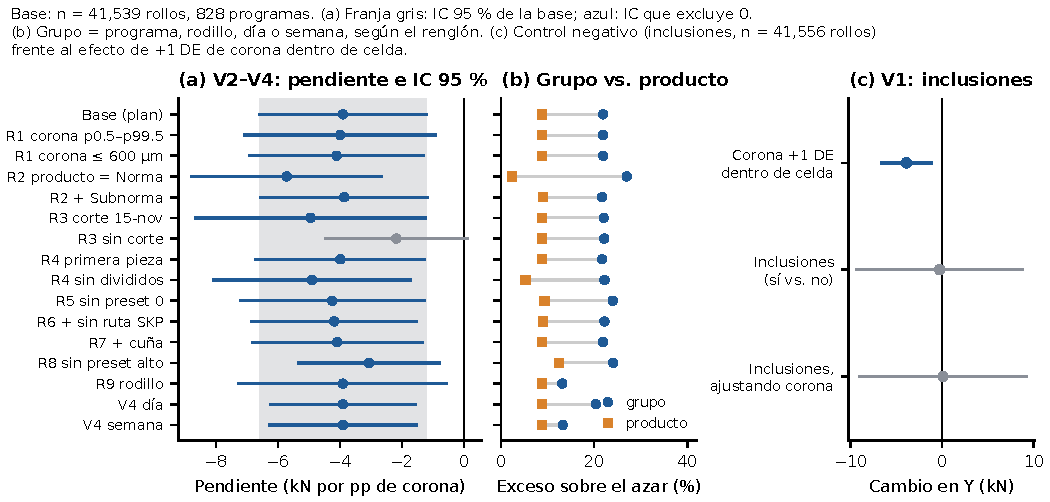
\includegraphics[width=\textwidth]{figuras/fig_r4_validacion.pdf}
\caption{\textbf{La dirección de la asociación y el predominio del programa sobre el producto sobreviven a
\NVariantes{} alternativas, y el control negativo no responde.} Pregunta que responde: ¿la conclusión depende de una
decisión de depuración, de la forma de agrupar o de una confusión que un control negativo detectaría? (a) Pendiente de
corona con su IC~95\,\% en cada alternativa (una sola decisión cambia por renglón; V4 agrupa la incertidumbre por día o
semana). (b) Exceso sobre el azar del grupo (programa, rodillo, día o semana) y del producto en la descomposición. (c)
Asociación de las inclusiones del MC4 con $\Y$, junto al efecto de una desviación estándar de corona.}
\label{fig:validacion}
\end{figure*}

\paragraph{V1, control negativo} Las inclusiones del MC4 (\NInclusiones{} rollos, \PctInclusiones\,\%) no se asocian
con la corrección: \VUnoCoef~kN \VUnoIC{} sin ajustar por la corona y \VUnoCoefAj~kN \VUnoICAj{} ajustando por ella
(Fig.~\ref{fig:validacion}c). El intervalo es amplio porque las inclusiones son raras; no excluye un efecto del tamaño
del de la corona, pero tampoco lo sugiere.

\paragraph{V2, consistencia física} El signo es el esperado (más corona, bending más negativo) y su intervalo excluye el
cero. La magnitud es pequeña: pasar del percentil 10 al 90 de la corona dentro de celda (de \VDosPdiez{} a
\VDosPnoventa~pp) cambia la corrección en \VDosCambio~kN, frente a una desviación estándar de \YDEAsoc~kN y un rango
intercuartil del bending real de \BendRealIQR~kN.

\paragraph{V3, robustez} Ninguna de las \NVariantes{} alternativas cambia el signo de la pendiente, que va de
\PendMvMin{} a \PendMvMax~kN por punto (Fig.~\ref{fig:validacion}a). Un intervalo, el de la alternativa sin corte de
censura, incluye el cero (\NVariantesICCero{} de \NVariantes): al incluir diciembre la pendiente se acerca a cero. En
todas las alternativas el grupo (programa, rodillo, día o semana) explica más que el producto
(Fig.~\ref{fig:validacion}b): el exceso del producto va de \ExcProdMvMin{} a \ExcProdMvMax~puntos y el del grupo de
\ExcGrupoMvMin{} a \ExcGrupoMvMax.

\paragraph{V4, programa contra periodo} Agrupar por día del Skinpass en lugar de por programa da casi lo mismo
(\VCuatroExcesoDia~puntos \VCuatroExcesoDiaIC, contra \VCuatroExcesoProg~\VCuatroExcesoProgIC{} del programa). Por
semana (\VCuatroExcesoSemana) y por rodillo de trabajo (\VCuatroExcesoRodillo) el exceso baja, pero sigue por encima
del producto (\VCuatroProductoProg).

\paragraph{Confusión no medida} El valor de robustez de la pendiente es de \CHRV\,\%: un confusor no medido que explique
esa proporción de la varianza residual de la corona y de la corrección bastaría para anularla (\CHRVa\,\% para que su
intervalo incluya el cero). El producto, el confusor observado de referencia, explica \CHRDRef\,\% de la varianza de la
corona y \CHRYRef\,\% de la de la corrección (dentro de dimensión y mes). Un confusor con solo \CHKAnula{} veces la fuerza
del producto, aproximadamente 1/\CHUnoEntre, bastaría para anular la pendiente.

\subsection{Predicción}
\label{sec:res-prediccion}

\begin{figure}[t]
\centering
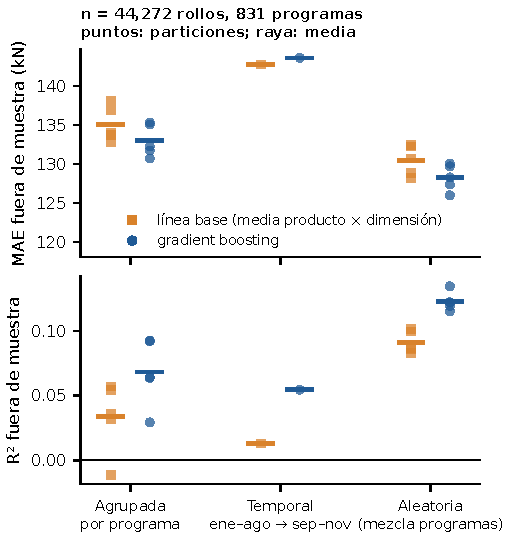
\includegraphics[width=\columnwidth]{figuras/fig_r5_prediccion.pdf}
\caption{\textbf{Con validación agrupada y temporal, el modelo no anticipa la corrección claramente mejor que una
receta por producto y dimensión.} Pregunta que responde: ¿la información disponible antes del Skinpass permite
anticipar $\Y$? Error absoluto medio (arriba) y $R^2$ fuera de muestra (abajo) de la línea base (media por producto
$\times$ dimensión) y del modelo, en cada partición. La validación aleatoria mezcla rollos de un mismo programa y se
muestra solo para ver cuánto infla el desempeño.}
\label{fig:prediccion}
\end{figure}

En las cinco particiones agrupadas por programa, el modelo baja el error absoluto medio de \PredMAEBaseGrupo{} a
\PredMAEModGrupo~kN (diferencia de \PredMAEDifGrupo~kN, DE \PredMAEDifGrupoDE{} entre particiones; mejora en
\PredMejoraGrupo{} de 5). En la partición temporal, entrenado con \PredNTempTrain{} rollos de enero a agosto y evaluado
en \PredNTempTest{} de septiembre a noviembre, el modelo es peor que la línea base en error absoluto medio
(\PredMAEModTemp{} contra \PredMAEBaseTemp~kN), aunque su $R^2$ es mayor (\PredRModTemp{} contra \PredRBaseTemp).
Por el criterio fijado antes de correrlo, no hay mejora clara. Ambos explican poco: el $R^2$ fuera de muestra del modelo
es de \PredRModGrupo{} en la validación agrupada (Fig.~\ref{fig:prediccion}). La validación aleatoria, que mezcla
rollos de un mismo programa, sube el $R^2$ de los dos (\PredRBaseAleat{} y \PredRModAleat). Lo que el modelo usa para
predecir es sobre todo el producto: permutarlo sube el error en \PredImpPrimeraKN~kN, contra \PredImpCorona~kN de la
corona, la segunda variable.

Por último, para dimensionar la propuesta de validación, estimamos con las mismas particiones agrupadas cuánto bajaría
el trabajo del lazo, $|\Y|$, si el preset se recentrara con la mediana histórica de la corrección. Con la receta
vigente, $|\Y|$ promedia \ExpAbsY~kN fuera de muestra; recentrar el preset por producto y dimensión lo bajaría
\ExpDeltaA~kN (DE \ExpDeltaADE{} entre particiones), y recentrarlo con una sola mediana global, \ExpDeltaGlobal~kN.
Diferenciar por producto agregaría \ExpDeltaDif~kN (DE \ExpDeltaDifDE) a recentrar la receta única.
